\chapter{Analýza}\label{ch:analýza}

\section{Bezpečnostné hrozby}\label{sec:podsekcia-1}
\par Z hľadiska bezpečnosti väčšina firiem čelí viacerým hrozbám.
V ideálnom prostredí a vo veľkých softvérových firmách slúži na analýzu bezpečnostných hrozieb takzvaný Systém riadenia
informačnej bezpečnosti(Information Security Management System - ISMS) podľa normy ISO 27000~\cite{ISO27001:2013}.
Úlohou takéhoto systému je definovanie a spravovanie rizík, ktoré môžu vyplývať z hrozieb a zraniteľností.
Dôležitou časťou je ochrana aktív s vysokou hodnotou.
Na obrázku~\ref{fig:obr_1} je možné vidieť schému riadenia takýchto rizík.

Medzi najzákladnejšie bezpečnostné problémy napríklad patrí nezabezpečený prístup k jednotlivým projektom medzi zamestnancami.
K jednotlivým projektom v softvérovej firme by mali mať prístup iba tí zamestnanci, ktorí sa podieľajú na jeho správe a implementácii.
Vystavenie prístupových údajov, rôznych informácií o zákazníkovi a jeho používateľoch neprislúchajúcemu zamestnancovi,
môže spôsobiť veľa bezpečnostných rizík.
Napríklad zamestnanec môže zneužiť dátové úložisko nachádzajúce sa v produkcii.
Zamestnanec môže týmto spôsobom  napríklad získať citlivé informácie o tržbách zákazníka alebo adrese.
Taktiež vie získať prístupové dáta k jeho koncovým zariadeniam a kompromitovať ich.
Týmto bezpečnostným rizikám prislúchajú aj možné následky nie len na strane softvérovej firmy.

\begin{figure}[H]
\begin{center}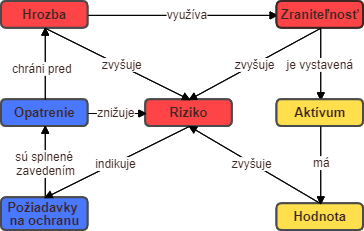
\includegraphics[width=\textwidth,height=6cm,keepaspectratio=true]{assets/risks.png}\end{center}
\caption[Prehľadová schéma riadenia rizík]{Prehľadová schéma riadenia rizík~\cite{RiskManagement}.}\label{fig:obr_1}
\end{figure}

Daný problém sa môže vyskytovať aj vo forme zlých právomocí k jednotlivým aktívam.
Softvérová firma teda môže mať navrhnutú výbornú izoláciu medzi jednotlivými projektami a zamestnancami.
Chybou môže byť aj neprimerané privilégium vo forme nadmerného prístupu k prostriedku.
Príkladom môže byť zamestnanec, ktorý nemá vo firme prístup k dátovému úložisku a jeho následnému upraveniu.
Ak nebol braný do úvahy aj prístup na prehliadanie jednotlivých údajov, takýto zamestnanec síce nevie dáta zmeniť alebo
vymazať, no je schopný prehliadať citlivé údaje a ich obsah zneužiť.

Medzi ďalšie problémy patrí takzvaná likvidácia dát.
Príkladom môže byť odchod zamestnanca z firmy.
Buďe mať stále po roku prístupy na jeho minulé projekty?
Bude mu prístup odobraný po ukončení pracovného pomeru?
Prípadne, čo ak na osobnom stretnutí prezradí prístupové údaje od bývalých projektov?
Je možné si tieto údaje útočníkom zapísať a následne sa dostať k prostriedkom?
Čo ak sa samotný zamestnanec bude chcieť po nečakanej výpovedi pomstiť napáchaním škôd?
V situácii, kedy zamestnanec nemá zrušené prístupové údaje, pričom bývalý projekt je nasadený a v praxi využívaný sa
jedná o veľmi veľké bezpečnostné riziko.

Ak sa jedná o manipuláciu so samotnými citlivými a prístupovými údajmi, tie môžu podliehať, ako bolo už spomínané neautorizovaným osobám.
Medzi najzákladnejšie riziká sú nekryptované, alebo nehašované citlivé dáta uložené v surovej forme na dátovom úložisku.
Príkladom využitia danej zraniteľnosti môže byť heslo používateľa.
Správca ani vlastník systému by nemal vedieť prístupové údaje používateľov v systéme.
Tu je možná forma zneužitia takýchto informácií k prístupu do používateľovho konta.
U systémov pracujúcich s finančnými prostriedkami, by mohlo ísť o krádež finančných prostriedkov používateľov vo vlastný prospech.

Prístup k vzdialeným zariadeniam zákazníka firmy by mala mať iba osoba, ktorá má na starosti nasadenie softvérového riešenia.
Keďže sa jedná o veľmi zodpovednú rolu vo firme, možnou hrozbou je zneužitie prístupových údajov odchytením pomocou útoku
MITM~\cite{MITM}, prípadne vyzradením údajov tretej strane podľahnutím phishing útoku~\cite{Phishing}.
Je možné sa chrániť aj proti takýmto hrozbám?

\begin{figure}[H]
\begin{center}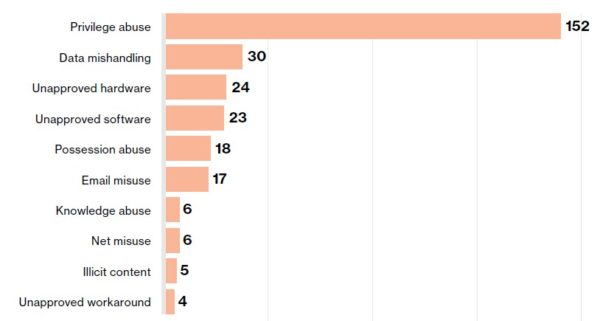
\includegraphics[width=\textwidth,height=6cm,keepaspectratio=true]{assets/priviledge_abuse.jpg}\end{center}
\caption[Najslabšie bezpečnostné miesta v softvérových firmách]{Najslabšie bezpečnostné miesta v softvérových firmách~\cite{WeaknestLink}.}\label{fig:obr_2}
\end{figure}

Ako môžme vidieť na obrázku~\ref{fig:obr_2}, najzraniteľnejším miestom v softvérových firmách je zneužitie práv zamestnancov.

\section{Súčasné opatrenia chrániace pred hrozbami}\label{sec:podsekcia-2}

Po vymenovaní konkrétnych hrozieb a možných rizík, ktoré z nich vyplývajú je dôležité zistiť formu súčasných riešení
protiopatrení, ktoré sú schopné možné riziká odstrániť, prípadne znížiť ich naplnenie.
V praxi je nutné finančne predpovedať náklady firmy vynaložené na opatrenie a finančne predpovedať náklady možného
následku po zneužití rizika.
Ak je napáchaná škoda zo zneužitia nižšia, ako dané protiopatrenie na zamedzenie takejto formy útoku, pre softvérovú
firmu a jej zákazníkov je zamedzenie takéhoto typu hrozby z pohľadu manažmentu neoptimálne.
Z takýchto, pre firmu nepodstatných rizík je vytvorený zoznam takzvaných zvyškových rizík, pričom ich znázornenie môžme
vidieť na obrázku~\ref{fig:obr_3}.

\begin{figure}[H]
\begin{center}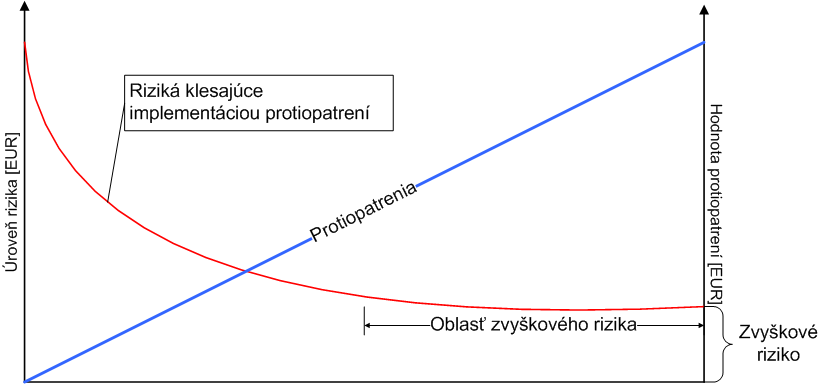
\includegraphics[width=\textwidth,height=6cm,keepaspectratio=true]{assets/zvyskove_riziko.png}\end{center}
\caption[Vizualizácia zvyškových rizík na základe hodnoty protiopatrení]{Vizualizácia zvyškových rizík na základe hodnoty protiopatrení~\cite{RiadenieRizik}.}\label{fig:obr_3}
\end{figure}

Priebeh celého procesu riadenia rizík sa vykonáva v nasledovných krokoch.
V prvom rade je nutné identifikovať riziko.
Druhým krokom je na základe druhu rizika vhodne stanoviť druh protiopatrenia.
Medzi možné spôsoby patria: Zníženie rizika, Presun rizika, Vyhnutie sa riziku, alebo zachovanie rizika.
Po validácii ošetreného rizika vznikajú podproblémy vo forme zvyškových rizík.
Tieto zvyškové riziká sú akceptované vtedy, ak nákladovosť na ich protiopatrenia sú vyššie, ako ich výška možných škôd.
Kontinuálne vykonávanie procesu riadenia rizík je možné znázorniť aj na upravenom Demingovom cykle (tzv\. model PDCA) z
bezpečnostnej normy ISO 27001.
Vykonávanie podľa daného modelu sa realizuje v štyroch fázach a to: Plánovať – Vykonávať – Kontrolovať – Pôsobiť.
Takýto model je možné prispôsobiť a upraviť pre potreby procesu riadenia rizík podľa obrázka~\ref{fig:obr_4} nasledovne.

\begin{figure}[H]
\begin{center}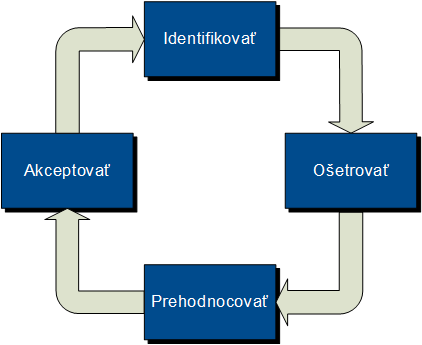
\includegraphics[width=\textwidth,height=6cm,keepaspectratio=true]{assets/pdca.png}\end{center}
\caption[Upravený PDCA model z normy ISO 27001]{Upravený PDCA model z normy ISO 27001~\cite{RiadenieRizik}.}\label{fig:obr_4}
\end{figure}

Po stručnom vysvetlení procesu riadenia rizík z pohľadu manažmentu informačnej bezpečnosti je na rade vysvetlenie
jednotlivých hrozieb spomenutých v predchádzajúcej časti práce.

Prvou hrozbou bol neautorizovaný prístup k aktívam neoprávnenými osobami.
Daný problém je z veľkej miery ovplyvnený vnútornou hierarchiou firmy.
Ak firma má v súčasnosti vytvorenú hierarchiu a každý zamestnanec má svoju špecifickú rolu na danom projekte, nutnosťou
pre zamedzenie výskytu rizík vyplývajúcich z danej hrozby je nasadenie systému autorizácie, ktorý bude jednotlivé roly
vo firme validovať, pričom prístup zamietne tým zamestnancom, ktorých rola nedovoľuje prístup k danému aktívu.

Jedným z najrelevantnejších (presne mapujúci danú hierarchiu firmy do systému) autorizačných modelov v súčasnej dobe, je riadenie prístupu na základe rolí (Role Based
Access Control - RBAC) podľa štandardu definovanom v ANSI/INCITS 359–2004~\cite{RBAC}.
Daný model je najčastejšie implementovaný ideológiou opatrnej bezpečnostnej politiky~\cite{OpatrnaBezpecnostnaPolitika},
ktorá spočíva v tom, že v systéme je zakázané všetko, čo nie je explicitne povolené.
Tým pádom si vieme model RBAC rozdeliť na dve časti.
Prvou je zoznam všetkých oprávnení, ktoré sú v systéme umožnené.
Druhou skupinou sú jednotlivé role, ktoré majú podľa ich významu zodpovedajúce oprávnenia.
RBAC implementácia spočíva v štyroch procesoch: Vytvorenie používateľa, vytvorenie role, priradenie role používateľovi,
a priradenie oprávnenia roli.
Jedným z problémov nastávajúcich v dynamických softvérových firmách sú výnimky vzhľadom na určité meniace sa podmienky.
Následkom výnimky vznikajú ďalšie role, ktorých počet môže byť časom neudržateľný,
pričom takto zneužité riešenie autorizovaného prístupu má za následok opätovné zvýšenie rizika zneužitia právomocí.
Jedným z možných riešení je vytvorenie dodatočnej tretej časti spočívajúcej vo vzťahu medzi samotným používateľom a oprávneniami.
Takýto vzťah by pre každého používateľa v systéme bol unikátny a nezávislý od jeho role, na rozdiel od mätúceho
vytvárania rozličných rolí s výnimkami.
Ďalšou výhodou takéhoto vzťahu je oddelenie medzi oprávneniami rolí a výnimkovými oprávneniami pre konkrétnych používateľov.

Medzi veľmi diskutované autorizačné metódy patrí riadenie prístupov na základe atribútov (Attribute-based access
control - ABAC), pričom kľúčový štandard, z ktorého ABAC vzišiel je XACML~\cite{XACML}.
Samotný koncept sa považuje za autorizačný model "novej generácie".
Dôvodom je iný spôsob prístupu k autorizačnej problematike.
Narozdieľ od RBAC udeľovanie prístupu používateľom sa riadi na základe jednotlivých aktív, inak povedané každej súčasti
systému~\cite{ABAC_RBAC_Attributes}.
Tento spôsob je veľmi užitočný, práve v spomínaných veľkých korporátnych softvérových firmách s veľmi výraznou dynamikou riadenia.
Pridelenie rolí používateľom teda naďalej nezávisí od ich role, ale od jednotlivých autorizačných pravidiel vyplývajúcich z namapovaných firemných aktív.
Týmto spôsobom je dokonca možné hodnotiť atribúty subjektov a zdrojov ešte pred ich zavedením do autorizačného systému.
Na druhej strane má daný koncept obmedzenie v konfigurácii, pričom určenie povolení daného používateľa je vzhľadom na návrh metódy veľmi obtiažne.
Pre danú bezpečnostnú problematiku, ktorou sa v práci zaoberáme vznikajú ďalšie nevýhody tohto riešenia a to náročnosť
implementácie a bezvýznamnosť danej metódy pre softvérové firmy menších rozmerov.
Na implementáciu daného konceptu je taktiež nutný podrobný návrh firemnej politiky~\cite{RBAC_ABAC_Encryption}.

Druhou hrozbou, ktorá so sebou prinášala veľký počet rizík bola otázka likvidácie dát.
Jednoduchým teoretickým riešením je všetky dáta a účty, ktoré už nie sú potrebné vymazať.
Realita vo firmách je žiaľ oveľa zložitejšia.
Ak zamestnanec z firmy odíde, neostane po ňom vo väčšine malých firiem iba jedno konto.
Tieto kontá a prístupové údaje bude nutné všetky vyhľadať, pričom sa vyskytujú na rôznych zariadeniach, službách technológiách a podobne.
Preto musí byť touto pracnou úlohou poverený zamestnanec z firmy, ktorému môže celý proces trvať niekoľko minút až hodín.
Takýto spôsob likvidácie dát je veľmi časovo náročný a hlavne obsahuje veľké riziko omylu a prehliadnutia niektorých z účtov.
Dané riziko nemusí explicitne vzísť iba z odchodu zamestnanca z firmy.
Zamestnancom sa počas pôsobenia v praxi môže meniť ich rola, projekty na ktorých pracujú, môže sa odstrániť služba,
ku ktorej musí mať prihlasovacie údaje a podobne.
Všetky tieto scenáre by mali byť riešené bezpečným, jednoduchým a centralizovaným spôsobom.

Jedným z riešení, ako sa vyhnúť daným rizikám je vytvorenie centrálnej autentifikácie zamestnancov.
Tým by sa zamedzilo udržiavaniu ich prihlasovacích údajov na viacerých miestach.
Jednou z možností je autentifikácia pomocou ľahkého protokolu prístupu k adresáru (Lightweight Directory Access Protocol - LDAP)~\cite{LDAP}.
Cieľom je vytvorenie servera, ktorý bude spravovať firemné prihlasovacie údaje jednotlivých zamestnancov, pričom
jednotlivé služby softvérovej firmy, ku ktorým je nutná autentifikácia budú podporovať autentifikáciu pomocou LDAP protokolu~\cite{LDAP_AUTH}.
Takéto riešenie by malo za následok správu všetkých kont zamestnancov na jednom mieste.
Ak by nastali popísané rizikové situácie, likvidácia dát je umožnená z jednoho centralizovaného bodu.
Priebeh autentifikácie na firemné aplikácie a služby by prebiehal podľa schémy na obrázku~\ref{fig:obr_5}.

\begin{figure}[H]
\begin{center}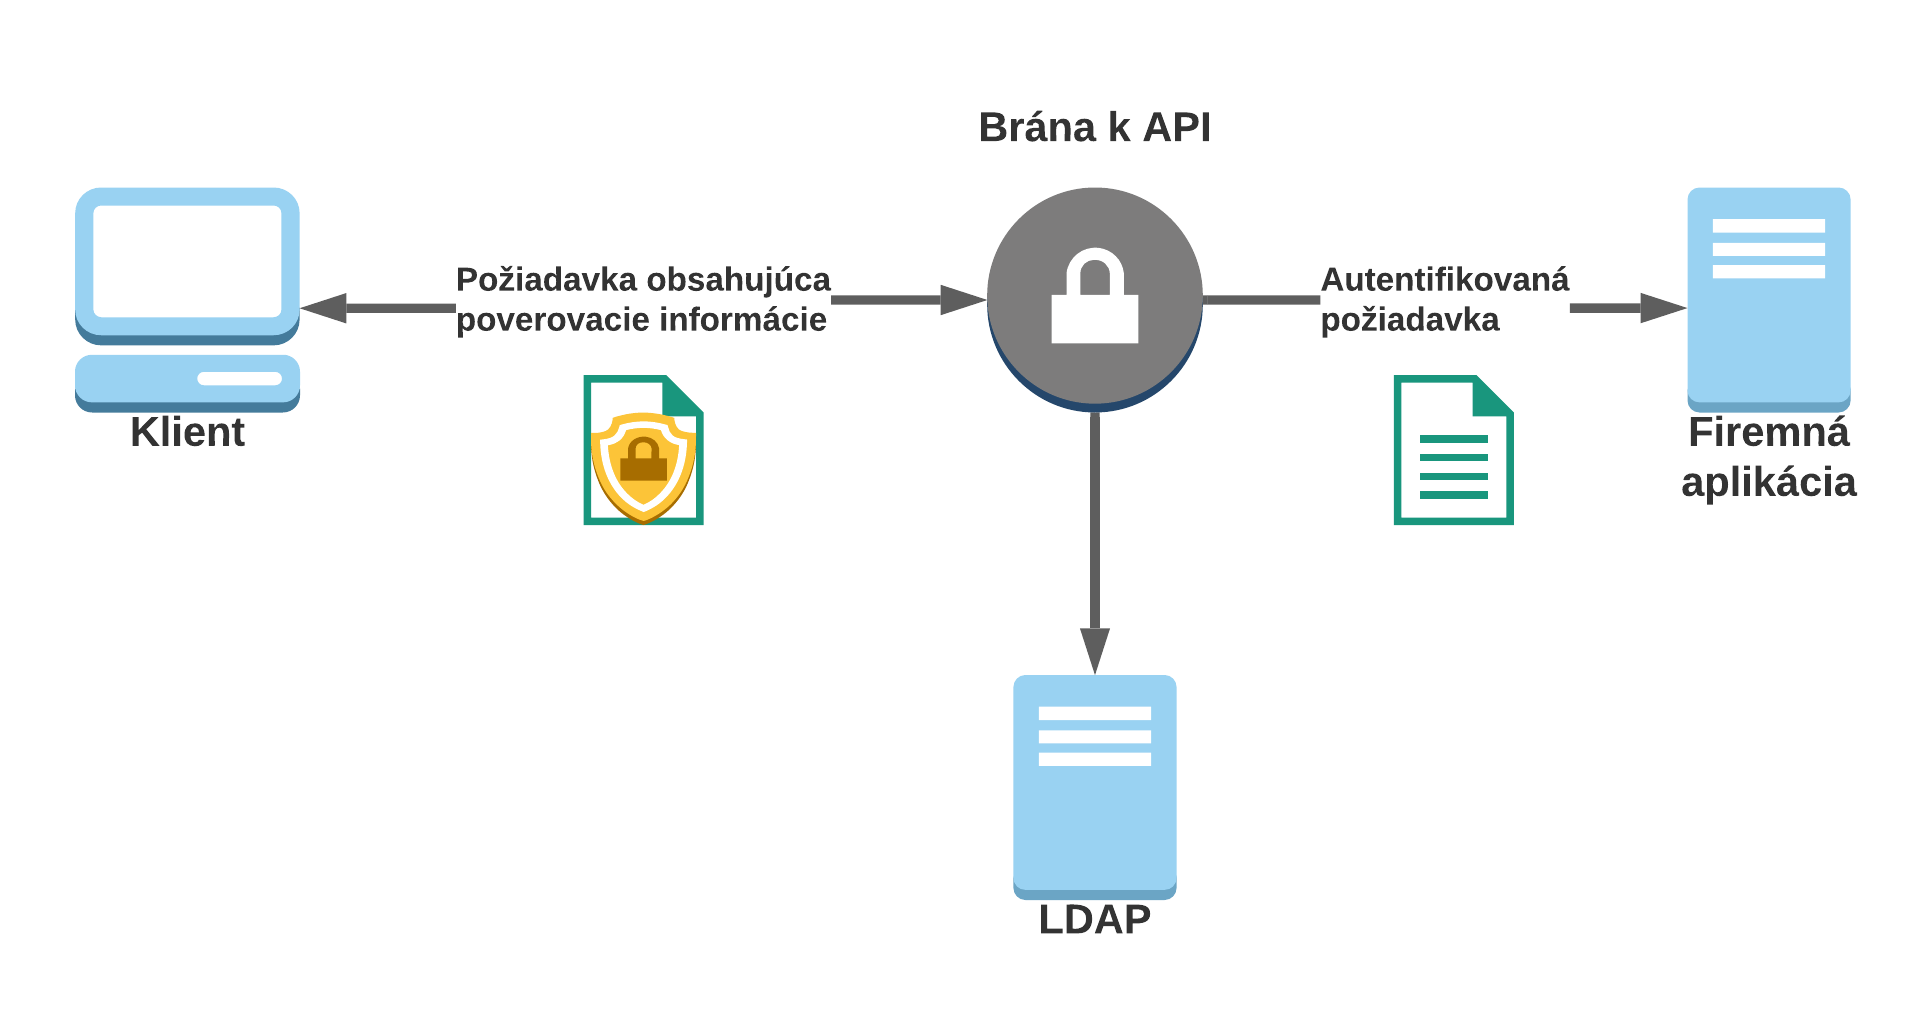
\includegraphics[width=\textwidth,height=6cm,keepaspectratio=true]{assets/ldap_schema.png}\end{center}
\caption[Schéma prihlasovania podľa protokolu LDAP]{Schéma prihlasovania podľa protokolu LDAP}\label{fig:obr_5}
\end{figure}

Treťou hrozbou bol prístup k dátam na dátovom úložisku.
Je možné dôverovať osobe s autorizáciou prehliadania dát s citlivými informáciami ako napríklad heslá, čísla kariet, prístupové adresy a podobne?
Na danú otázku existuje odpoveď vo forme modelu CIA, známeho aj ako model rozvoja bezpečnostnej politiky~\cite{CIA}.
Skratka CIA hovorí o troch dôležitých bezpečnostných pilieroch manipulácie s dátami.
Prvým z nich dôvernosť (Confidentality), ktorý hovorí o neschopnosti zistenia obsahu dôverných informácií ktorýmkoľvek používateľom.
Ako chceme dôverné informácie ochrániť pred všetkými zamestnancami, aj tými, ktorí majú k dátovému úložisku nutnú autorizáciu?
Bezpečnými spôsobmi ochrany informácií sú enkrypcia a hašovanie.
Enkrypcia je v skratke obojsmerná funkcia.
Tým pádom slúži na anonymizovanie statických dát ako napríklad informácie umožňujúce identifikáciu osôb~\cite{Encryption}.
Konkrétne sa môže jednať o dáta typu: Číslo vodičského preukazu, číslo občianskeho preukazu a podobne.
Na druhej strane hašovacia funkcia je jednosmerná.
Inak povedané, funkcia nemá možnosť spätného "odhašovania" informácie~\cite{Hashing}.
Bezpečným prvkom, ktorý je k hašovaniu možné pridať je takzvaný "salt", ktorý danú hašovaciu funkciu zamieša špecifickým reťazcom znakov.
Hašovacia funkcia sa používa pri druhoch informácií, ktoré sú posielané medzi dvomi sieťovými bodmi.
Napríklad môže ísť o heslo, ktorého reálnu hodnotu nikdy na strane zariadenia ktoré ho uchováva nemusíme vedieť.
Stačí, ak sa rovnaký spôsob hašovania hesla použije na strane zariadenia vyžadujúceho autentifikáciu.
Pri procese autentifikácie sa oba haše porovnajú a ak sa rovnajú, heslá sa zhodujú.
Výsledkom hašovacej funkcie je fixne dlhý reťazec znakov.
Napríklad pri texte dlhom 250 znakov môže byť výsledný haš dlhý 32 znakov.
Preto dôležitým atribútom hašovacích funkcií je ich matematicky veľmi nízka pravdepodobnosť na vytvorenie dvoch rovnakých
výstupných reťazcov pri rozdielnych vstupoch.
Druhým pilierom modelu CIA je integrita (Integrity), ktorá hovorí o konzistencii informácií na dátovom úložisku.
Ak by došlo k ich modifikácii, vlastník daných informácií musí byť informovaný o ich zmene.
Táto skutočnosť vie ochrániť vlastníkov údajov pred ich nežiadúcou zmenou, ktorá môže byť spôsobená neautorizovaným prístupom.
Posledným pilierom modelu CIA je dostupnosť (Availability).
K skutočnej forme informácií môže mať prístup iba ich vlastník a to v čitateľnej a konečnej podobe.
To napríklad znamená, že pred zobrazením používateľovho rodného čísla musí byť táto enkryptovaná dôverná informácia
spätne dekryptovaná do originálnej podoby.

Posledný spomínaný problém nesie so sebou výskyt rizík v podobe získania prístupových údajov, či už sa jedná o autentifikáciu
do firemného systému, alebo dáta potrebné na nasadenie finálneho softvérového produktu ku koncovým zariadeniam zákazníkov.
V oboch prípadoch, ako bolo už spomenuté ide o veľmi vážne bezpečnostné riziká, keďže sa taktiež priamo týkajú zákazníkov
softvérovej firmy.
Pre šifrovaný spôsob komunikácie je potrebné implementovať komunikačné protokoly v súlade s bezpečnostnými požiadavkami.
Komunikácia medzi vzdialeným webovým firemným serverom a zamestnancom by mohla prebiehať cez zabezpečený protokol
HTTPS (Hypertext transfer protocol secure)~\cite{HTTPS}, kde by boli jednotlivé autentifikačné dáta na transportnej vrstve
šifrované bezpečnostným protokolom TLS (Transport Layer Security)~\cite{TLS}.
Samotný spôsob autentifikácie by mohol byť uskutočnený podľa formátu JWT (JSON Web Token) spolu s využitím autentifikačného
protokolu OAUTH(2.0) (Open standard for access delegation)~\cite{JWT}.
Keďže prístup k firemným zdrojom je veľmi diskrétny, z bezpečnostného hľadiska je odporúčané použitie dvojfaktorovej
autentifikácie~\cite{DvojfaktorovaAutentifikacia}, ktorej priebeh môžme vidieť na obrázku~\ref{fig:obr_6}.
Dvojfaktorová autentifikácia nepodlieha útokom hrubou silou a taktiež po získaní prístupových dát napríklad odchytením,
alebo inou formou útoku nepodlieha ich zneužitiu z dôvodu veľmi frekventovane meniaceho sa unikátneho verifikačného kódu.
Pokiaľ sa jedná o komunikáciu medzi koncovými zariadeniami zákazníkov, tú je možné zabezpečiť protokolom SFTP (SSH File
Transfer Protocol)~\cite{SFTP}, ktorý umožňuje posielanie súborov cez protokol SSH (Secure Shell)~\cite{SSH}, slúžiaci
na bezpečné vykonávanie príkazov na vzdialených zariadeniach.

\begin{figure}[H]
\begin{center}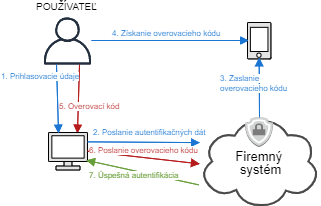
\includegraphics[width=\textwidth,height=6cm,keepaspectratio=true]{assets/auth.png}\end{center}
\caption[Schéma dvojfaktorovej autentifikácie]{Schéma dvojfaktorovej autentifikácie}\label{fig:obr_6}
\end{figure}

\section{Zhodnotenie}\label{sec:podsekcia-3}

Z analýzy vyplýva, že jednotlivé problémy spojené s bezpečnostnými rizikami sú v súčastnosti riešiteľné veľkým počtom
rôznych spôsobov protiopatrení.
Taktiež existujú presne špecifikované postupy a normy, ktoré je dôležité dodržovať softvérovými firmami pre zlepšenie
ich informačnej bezpečnosti.
Otázkou ostáva, z akého dôvodu naďalej väčšina malých softvérových firiem odkladá, alebo úmyselne prehliada jednotlivé bezpečnostné hrozby.
V prvom rade je dôležité si uvedomiť, že firmy sú schopné jednotlivé bezpečnostné opatrenia vyriešiť, no z dôvodu
prekážok, v podobe časových a finančných prostriedkov im vo väčšine prípadov takáto možnosť riešenia nie je umožnená~\cite{CompanySecurity}.
Príkladom môže byť nízky počet zamestnancov, ktorý sú potrebný na jednotlivých špecializovaných úlohách  pridelených k projektom.
Prevelením jednoho zamestnanca z projektu s cieľom riešenia firemnej bezpečnosti, môže mať za následok rapídne zníženie
produktivity na určitých častiach práce.
Ďalším reálnym problémom je financovanie časovo náročných bezpečnostných opatrení, ktorých implementácia je financovaná priamo z firemného rozpočtu.
Jedným z finančne a časovo nenáročných riešení pre softvérové firmy pramení z idei spojenia všetkých analyzovaných
bezpečnostných opatrení do jednoho celku, v podobe informačného bezpečnostného systému.
Takýto systém by obsahoval všetky bezpečnostné aspekty protiopatrení, pričom jeho návrh a implementácia by sa musela prioritne riadiť podľa kritérií vysokej
bezpečnosti, modularity a rozšíriteľnosti.
Dôvodom je použitie implementovaného bezpečnostného riešenia v praxi jednotlivými firmami ako produktu tretej strany,
pričom firmy by mohli podľa ich potrieb jednotlivé časti systému ľahko upraviť, prípadne doplniť o nové bezpečnostné prvky.

% TODO: porovnanie existujucich rieseni (ako to robi amazon google atd.)
% TODO: zhodnotenie a porovnanie ci to ma zmysel ci ne atd.
